\documentclass[13pt,oneside]{book}
\usepackage[utf8]{inputenc}
\usepackage{url}
\usepackage{listings}
\usepackage{graphicx}

\usepackage{geometry}
\geometry{a4paper, left=20mm, right=20mm, top=20mm, bottom=20mm}
\usepackage[margin=1.2in]{geometry}
\usepackage[toc,page]{appendix}
\usepackage{graphicx}
\usepackage{natbib}
\usepackage{lipsum}
\usepackage{caption}

\begin{document}

\captionsetup[figure]{margin=1.5cm,font=small,labelfont={bf},name={Figure},labelsep=colon,textfont={it}}
\captionsetup[table]{margin=1.5cm,font=small,labelfont={bf},name={Table},labelsep=colon,textfont={it}}
\setlipsumdefault{1}

\begin{titlepage}
\begin{center}
{\LARGE College Of Engineering Trivandrum}\\[3cm]
\linespread{1.2}\huge {\bfseries System Software Lab}\\[3cm]
\linespread{1}

\includegraphics[width=5cm]{img/emblem.jpeg}\\[3cm]
{\Large GOKUL K\\ S5  CSE \\ Roll No:21\\ TVE18CS021 }\\[1cm]


\textit{ }\\[2cm]
Department of Computer Science\\[0.2cm]
\today
\end{center}

\end{titlepage}

\newpage

\begin{frame}{}
    \centering
    \hspace*{-0.5cm}
    $\vcenter{\hbox{
\includegraphics[width=1.5cm]{img/emblem.jpeg}}}$
    $\vcenter{\resizebox{0.95\textwidth}{!}{
        \begin{tabular}{c}
             CS331 - System Software Lab $\cdot$ 2020 $\cdot$   \\
             \hline 
        \end{tabular}
    }}$
\end{frame}
\section*{Cycle 1}
\section*{Expt 1}
\begin{center}
    \Large{CPU Scheduling Algorithms}
\end{center}

\section*{Aim}
\large{
Simulate the following non-preemptive CPU Scheduling
Algorithms to find turnaround time and waiting time.\\
a) FCFS\\
b) SJF\\
c) Round Robin (pre-emptive)\\
d) Priority\\
}

\section*{Algorithm}
    \subsection*{FCFS}
	    \begin{verbatim}
	        1 Start .
            2 Input the processes along with their burst time ( bt ) and
                arrival time ( at ) .
            3 Find the waiting time ( wt ) for all processes .
            4 As process that arrives first need not wait , wt for that process
                will be 0 , wt [0] = 0.
            5 Calculate the wt for all other processes as :
            6 For process i , wt [ i ] = 
                ( bt [0] + bt [1] + .... + bt [i -1]) - at [ i ]
            7 Find turnaround time ( tat ) for all processes .
            8 For process i , tat [ i ] = wt [ i ] + bt [ i ]
            9 Compute average waiting time as ( total_wt / no_of_processes ) .
            10 Compute average turnaround time as ( total_tat / no_of_processes ) .
            11 Stop .
	   \end{verbatim}  
    \subsection*{SJF}
        \begin{verbatim}
            1 Start
            2 Input the processes along with their burst time ( bt ) .
            3 Sort the processes in ascending order of their burst times .
            4 Find the waiting time ( wt ) for all processes .
            5 As the process with smallest bt is scheduled first , it need
                not wait ,
            6 so wt for that process will be 0 , wt [0] = 0.
            7 Calculate the wt for all other processes as :
            8 For process i , wt [ i ] = wt [i -1] + bt [i -1]
            9 Find turnaround time ( tat ) for all processes .
            10 For process i , tat [ i ] = wt [ i ] + bt [ i ]
            11 Compute average waiting time as ( total_wt / no_of_processes ) .
            12 Compute average turnaround time as ( total_tat / no_of_processes ) .
            13 Stop .
        \end{verbatim}  
        
    \subsection*{Round Robin}
        \begin{verbatim}
            1 Start
            2 Input the processes along with their burst time ( bt ) .
            3 Input the time quantum , tq .
            4 Create an array rem_bt [] to keep track of the remaining burst time
                of processes . This array is initially a copy of bt [].
            5 Create another array wt [] to store the waiting times of processes .
            6 Initialize this array as 0.
            7 Initialize time t = 0.
            8 Keep traversing all the processes while all processes are not done
                yet . Do the following for the i th process if it is not done yet
            9 If rem_bt [ i ] > tq
            10 t = t + tq
            11 rem_bt [ i ] = tq
            12 Else
            13 t = t + rem_bt [ i ]
            14 wt [ i ] = t - bt [ i ]
            15 rem_bt [ i ] = 0
            16 // Last cycle for this process
            17 // This process is over
            18 Find turnaround time ( tat ) for all processes .
            19 For process i , tat [ i ] = wt [ i ] + bt [ i ]
            20 Compute average waiting time as ( total_wt / no_of_processes ) .
            21 Compute average turnaround time as ( total_tat / no_of_processes ) .
            22 Stop .
        \end{verbatim}
        
    \subsection*{Priority}
        \begin{verbatim}
            1 Start .
            2 Input the processes along with their burst time ( bt ) and priority .
            3 Sort the processes in ascending order of their priorities .
            4 Find the waiting time ( wt ) for all processes .
            5 As the process with highest priority is scheduled first , it need
                not
            6 wait , so wt for that process will be 0 , wt [0] = 0.
            7 Calculate the wt for all other processes as :
            8 For process i , wt [ i ] = wt [i -1] + bt [i -1]
            9 Find turnaround time ( tat ) for all processes .
            10 For process i , tat [ i ] = wt [ i ] + bt [ i ]
            11 Compute average waiting time as ( total_wt / no_of_processes ) .
            12 Compute average turnaround time as ( total_tat / no_of_processes ) .
            13 Stop .
        \end{verbatim}
\section*{Source Code}
\Large\textbf{process.c}
\small

\begin{lstlisting}[language=C]
#include <stdio.h>
#include <stdlib.h>
#include "process.h"

Process_ptr read_process()
{
	Process_ptr process_ptr = malloc(sizeof(Process));
	scanf(
		"%d %d %d %d", 
		&(process_ptr->p_num),
		&(process_ptr->arrival_time),
		&(process_ptr->execute_time),
		&(process_ptr->priority)
	);
	process_ptr->turnaround_time = process_ptr->waiting_time = 0;
	process_ptr->rem_time = process_ptr->execute_time;
	return process_ptr;
}

Process_list * read_process_list()
{
	/* The list must be sorted by arrival time.
	Hence insertion sort is used */
	size_t length, i;
	short int j;
	Process_ptr key, process_itr;
	Process_ptr *processes;
	Process_list *process_list = malloc(sizeof(Process_list));

	printf("Enter number of processes: ");
	scanf("%d", &(process_list->length));

	process_list->processes = malloc(
	    process_list->length * sizeof(Process_ptr *)
	);
	processes = process_list->processes;

	printf("\nEnter process number, arrival time, execution time and
	priority"
	"\nfor the process. Each value must be seperated by a space\n");
	for(i = 0; i < process_list->length; ++i)
	{
		printf("Process%d: ", i);
		*(processes+i) = read_process();
		key = *(processes+i);
		
		j = i-1;

		while(j >= 0 && 
		    processes[j]->arrival_time > key->arrival_time)
		{
			process_itr = *(processes+j);

			*(processes+j+1) = process_itr;
			--j;
		}
		*(processes+j+1) = key;
	}

	return process_list;
}

void comp_avg_times(Process_list * process_list)
{
	float avg_turnaround_time = 0.0;
	float avg_waiting_time = 0.0;

	for(size_t i = 0; i < process_list->length; i++)
	{
		avg_turnaround_time += 
		    process_list->processes[i]->turnaround_time;
		avg_waiting_time += 
		    process_list->processes[i]->waiting_time;
	}

	avg_turnaround_time /= process_list->length;
	avg_waiting_time /= process_list->length;

	printf(
		"\nAverage waiting time: %.2fu"
		"\nAverage turn-around time: %.2fu\n",
		avg_waiting_time,
		avg_turnaround_time
	);
}

int comp_total_rem_time(Process_list * process_list)
{
	int rem_time = 0;
	for(size_t i = 0; i < process_list->length; i++)
	{
		rem_time += process_list->processes[i]->rem_time;
	}
	return rem_time;
}

    \end{lstlisting}
    
\Large\textbf{schedule.c}
\small
\begin{lstlisting}[language=C]
#include "process.h"
#include <stddef.h>
#include <stdio.h>

void draw_gantt_cell(int p_num, int second, int start_cell, int end_cell) {
  if (start_cell)
    printf("\nGantt Chart (Not-to-scale): ");

  printf("\n----------   t=%du", second);
  printf("\n|P%*d|", 8, p_num);

  if (end_cell)
    printf("\n----------   t=%du\n\n", end_cell);
}

int fcfs(Process_list *process_list) {
  size_t i;
  Process_ptr process_ptr;
  int curr_time = process_list->processes[0]->arrival_time;

  for (i = 0; i < process_list->length; ++i) {
    process_ptr = process_list->processes[i];

    draw_gantt_cell(process_ptr->p_num, curr_time, i == 0,
                    (i == process_list->length - 1)
                        ? curr_time + process_ptr->execute_time
                        : 0);

    process_ptr->waiting_time = curr_time - process_ptr->arrival_time;
    process_ptr->turnaround_time =
        process_ptr->waiting_time + process_ptr->execute_time;
    process_ptr->rem_time = 0;
    curr_time += process_ptr->execute_time;
  }
}

int sjf(Process_list *process_list) {
  size_t i, j;
  Process_ptr process_ptr, process_itr;

  int curr_time = process_list->processes[0]->arrival_time;
  for (i = 0; i < process_list->length; ++i) {
    process_ptr = process_list->processes[i];
    for (j = 0; j < process_list->length; j++) {
      process_itr = process_list->processes[j];
      if (!(process_ptr->rem_time) ||
          process_itr->rem_time && process_itr->arrival_time <= curr_time &&
              process_itr->execute_time < process_ptr->execute_time) {
        process_ptr = process_itr;
      }
    }

    draw_gantt_cell(process_ptr->p_num, curr_time, i == 0,
                    (i == process_list->length - 1)
                        ? curr_time + process_ptr->execute_time
                        : 0);
    process_ptr->waiting_time = curr_time - process_ptr->arrival_time;
    process_ptr->turnaround_time =
        process_ptr->waiting_time + process_ptr->execute_time;
    process_ptr->rem_time = 0;
    curr_time += process_ptr->execute_time;
  }
}

int round_robin(Process_list *process_list, int quantum_time) {
  int total_rem_time = comp_total_rem_time(process_list);
  int instant_work_done, curr_time = 0;

  int last_processed_time[process_list->length];
  Process_ptr process_ptr;
  size_t i;

  // Initialize with all zero
  for (i = 0; i < process_list->length; ++i)
    last_processed_time[i] = 0;

  while (total_rem_time > 0) {
    for (i = 0; i < process_list->length; i++) {
      process_ptr = process_list->processes[i];
      if (!process_ptr->rem_time)
        continue;

      instant_work_done = (process_ptr->rem_time > quantum_time)
                              ? quantum_time
                              : process_ptr->rem_time;
      total_rem_time -= instant_work_done;
      process_ptr->rem_time -= instant_work_done;
      draw_gantt_cell(
          process_ptr->p_num, curr_time, curr_time == 0,
          (total_rem_time == 0 ? curr_time + instant_work_done : 0));
      process_ptr->waiting_time += curr_time - last_processed_time[i];
      process_ptr->turnaround_time +=
          curr_time - last_processed_time[i] + instant_work_done;

      curr_time += instant_work_done;
      last_processed_time[i] = curr_time;
    }
  }
}

int priority(Process_list *process_list) {
  size_t i, j;
  Process_ptr process_ptr, process_itr;

  int curr_time = process_list->processes[0]->arrival_time;
  for (i = 0; i < process_list->length; ++i) {
    process_ptr = process_list->processes[i];  
    for (j = 0; j < process_list->length; j++) {
      process_itr = process_list->processes[j];
      if (!(process_ptr->rem_time) ||
          process_itr->rem_time && process_itr->arrival_time <= curr_time &&
              process_itr->priority < process_ptr->priority) {
        process_ptr = process_itr;
      }
    }

    draw_gantt_cell(process_ptr->p_num, curr_time, i == 0,
                    (i == process_list->length - 1)
                        ? curr_time + process_ptr->execute_time
                        : 0);
    process_ptr->waiting_time = curr_time - process_ptr->arrival_time;
    process_ptr->turnaround_time =
        process_ptr->waiting_time + process_ptr->execute_time;
    process_ptr->rem_time = 0;
    curr_time += process_ptr->execute_time;
  }
}
\end{lstlisting}
\Large\textbf{main.c}
\small
\begin{lstlisting}[language=C]
#include <stdio.h>

#include "process.h"
#include "schedule.h"


int main()
{
	int quantum_time, choice;
	Process_list * process_list = read_process_list();

	printf(
		"Select the scheduling algorithm:"
		"\n\t1) First Come First Serve"
		"\n\t2) Shortest Job First"
		"\n\t3) Round Robin (pre-emptive)"
		"\n\t4) Priority\n"
	);
	scanf("%d", &choice);
	switch (choice)
	{
		case 1:
			fcfs(process_list);
			break;

		case 2:
			sjf(process_list);
			break;
		
		case 3:
			printf("\nEnter quantum time: ");
			scanf("%d", &quantum_time);
			round_robin(process_list, quantum_time);
			break;

		case 4:
			priority(process_list);
			break;

		default:
			break;
	}

	comp_avg_times(process_list);
}

\end{lstlisting}
\section*{Output}
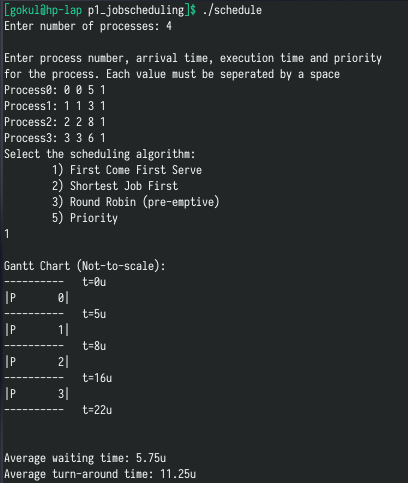
\includegraphics[]{img/p1/ss1.png} \\
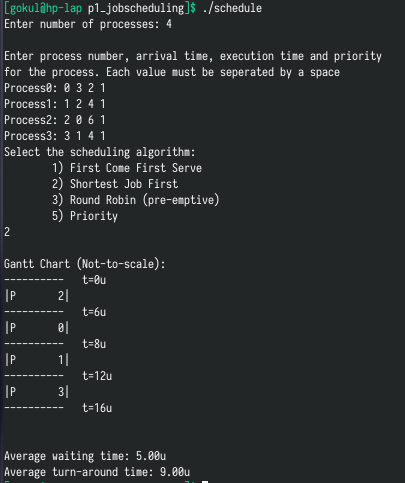
\includegraphics[]{img/p1/ss2.png} \\
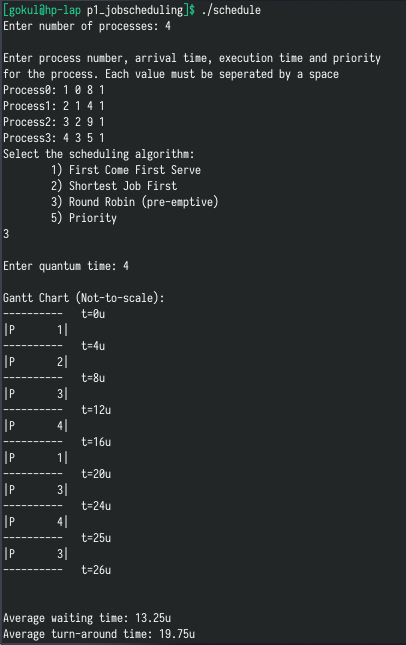
\includegraphics[]{img/p1/ss3.png} \\
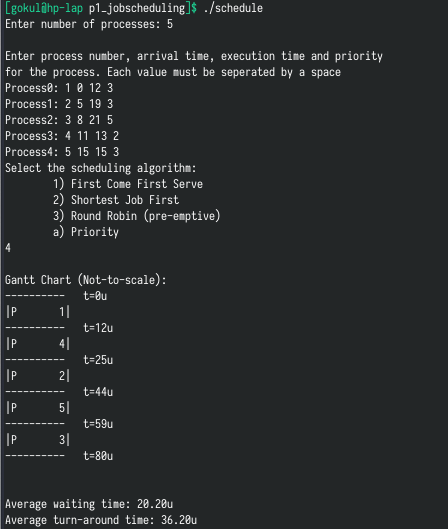
\includegraphics[]{img/p1/ss4.png}

\Large
\section*{Result}
\large
The above algorithms were implemented and its output verified

\end{document}